\documentclass[]{imag-ms-template}

%the class loads mathtools, amssymb, booktabs, graphicx, biblatex (APA, natbib commands) and hyperref
\usepackage[utf8]{inputenc}
\usepackage[T1]{fontenc}
\usepackage{lmodern}
\IfFileExists{microtype.sty}{\usepackage{microtype}}{}
\usepackage{multirow}
\usepackage{xcolor}
\usepackage{tikz}
\usetikzlibrary{calc,decorations.pathreplacing,calligraphy,shapes.geometric,intersections}
\usepackage{caption}
\usepackage{subcaption}
\usepackage{placeins}
\usepackage{lineno}
\usepackage{xr}
\externaldocument[S-]{supplementary}
\linenumbers
%let figures and tables share pages with text instead of leaving half-empty float pages
\renewcommand{\topfraction}{0.9}\renewcommand{\bottomfraction}{0.8}\renewcommand{\textfraction}{0.07}\renewcommand{\floatpagefraction}{0.8}
\hypersetup{colorlinks=true,linkcolor=blue!50!black,citecolor=blue!50!black,urlcolor=blue!50!black}
\addbibresource{references.bib}

%points the authors must check before submission
\newcommand{\TBD}[1]{\textcolor{red}{[#1]}}
\newcommand{\E}{\mathbb{E}}
\newcommand{\R}{\mathbb{R}}
%\input is not expandable inside tabular (misplaced \noalign before \bottomrule); the TeX primitive is
\makeatletter\newcommand{\tabinput}[1]{\@@input #1.tex }\makeatother
%auto-generated by make_tables.py; do not edit
\newcommand{\ridgeEEGvsECG}{0.00}
\newcommand{\ridgeEEGvsMOTION}{0.02}
\newcommand{\ridgeEEGvsHR}{0.64}

%auto-generated by make_tables.py; do not edit
\newcommand{\sesoiNLL}{0.104}
\newcommand{\sesoiCRPS}{0.011}
\newcommand{\sesoiRMSE}{0.023}


\title{Uncertainty Confounds in EEG-to-fMRI Synthesis}

\author{David Calhas,$^{1\ast}$ Rui Henriques$^{2}$\\
{\small $^{1}$Faculty of Computer and Information Science, University of Ljubljana, Ljubljana, Slovenia}\\
{\small $^{2}$INESC-ID, Instituto Superior T\'{e}cnico, Universidade de Lisboa, Lisbon, Portugal}\\
{\small $^\ast$Correspondence: David Calhas, david.calhas@fri.uni-lj.si}
}
\date{}

\begin{document}
\maketitle

\keywords{simultaneous EEG--fMRI; EEG-to-fMRI synthesis; uncertainty quantification; physiological confounds; conformal prediction}

\begin{abstract}
Deep networks that synthesize functional magnetic resonance imaging (fMRI) from simultaneously recorded electroencephalography (EEG) are increasingly paired with uncertainty estimates, but likelihood, coverage and error--uncertainty correlation cannot show that an estimate is about the EEG. We propose an EEG-conditional evaluation that compares every model with EEG-free predictive distributions, re-scores it with its EEG shifted in time or taken from another subject, and injects a known EEG-coupled signal as a positive control. Applied to multiple uncertainty quantification methods on simultaneous EEG--fMRI from 17 subjects, it shows that no method is significantly better than a voxelwise template fitted without EEG, and that the predicted uncertainty of every method is a static anatomical map, identical whatever EEG is supplied. The positive control explains why: the heteroscedastic training most methods share makes the network ignore its input, while the same backbone trained with a point loss recovers the injected signal ($r=0.48$, ceiling 0.71). Models that are sensitive find no subject-specific EEG information beyond the shared task timing. At the region level, a lagged EEG model predicts motor BOLD across subjects and passes a published surrogate test, but heart rate from the in-scanner electrocardiogram (ECG) predicts it as well, and across subjects the EEG adds nothing to heart rate and motion. The results replicate on a second cohort. Our results suggest that calibrated uncertainty and surrogate-tested prediction are not evidence of neural information, and we need EEG-free references, subject-swap nulls, physiological confounds and positive controls to show it.
\end{abstract}

\section{Introduction}\label{sec:introduction}
A model that predicts functional magnetic resonance imaging (fMRI) from electroencephalography (EEG) would give access to haemodynamic information at the cost and in the settings of an EEG recording. Deep synthesizers \citep{liu2019convolutional,calhas2022eeg,li2024neurobolt} have been proposed for this, and for any clinical use their predictions need an uncertainty estimate \citep{begoli2019need}. Uncertainty quantification (UQ) can be done through heteroscedastic likelihoods \citep{kendall2017uncertainties}, approximate Bayesian weights \citep{blundell2015weight,gal2016dropout,maddox2019simple,daxberger2021laplace}, ensembles \citep{lakshminarayanan2017simple} and conformal intervals \citep{lei2018distribution,romano2019conformalized}. 

EEG-to-fMRI synthesis is an unusual setting for these tools. Most of the variance of an fMRI volume is anatomy shared across subjects, learnable without the EEG, and the part that varies in time also follows the heart and head motion, which leak into the EEG \citep{friston1996movement,power2014methods}. A predictive distribution can therefore be calibrated, its spread can track its error, and its mean can pass a surrogate test, while it carries no neural information from the EEG. The standard checks never ask what they give without the input. \citet{liu2019convolutional} first mapped EEG to fMRI volumes with a convolutional network, and \citet{calhas2022eeg} proposed the encoder we use. In medical imaging, uncertainty has been studied for segmentation \citep{mehrtash2020confidence}, reconstruction \citep{narnhofer2021bayesian} and diffusion MRI \citep{tanno2021uncertainty}, where the target is mostly determined by the input, so whether the uncertainty depends on the input need not be asked. Our protocol carries the negative controls of neuroimaging machine learning \citep{varoquaux2018cross,kapoor2023leakage,schreiber1996improved} over to predictive uncertainty.

\begin{figure}[!htbp]
    \centering
    
    \begin{tikzpicture}
        [scale=1.2, inner sep=3mm,
        in_node/.style={circle, draw=red!90, fill=red!20,thick,inner sep=0pt, minimum size=3mm},
        out_node/.style={circle, draw=blue!90, fill=blue!20,thick,inner sep=0pt,minimum size=3mm}]
            
        
        %draw model 1st model
        %in nodes
        \node (1stinnode) at (0,0) [in_node] {};
        \node (2ndinnode) at ($(1stinnode)+(0.5,0)$) [in_node] {};
        \node (3rdinnode) at ($(2ndinnode)+(0.5,0)$) [in_node] {};
        %out nodes
        \node (3rdoutnode) at ($(2ndinnode)+(0,1)$) [out_node] {};
        \node (1stoutnode) at ($(3rdoutnode)+(-1,0)$) [out_node] {};
        \node (2ndoutnode) at ($(1stoutnode)+(0.5,0)$) [out_node] {};
        \node (3rdoutnode) at ($(2ndoutnode)+(0.5,0)$) [out_node] {};
        \node (4thoutnode) at ($(3rdoutnode)+(0.5,0)$) [out_node] {};
        \node (5thoutnode) at ($(4thoutnode)+(0.5,0)$) [out_node] {};
        %fully connect nodes
        \draw[->] (1stinnode) -- (1stoutnode);
        \draw[->] (1stinnode) -- (2ndoutnode);
        \draw[->] (1stinnode) -- (3rdoutnode);
        \draw[->] (1stinnode) -- (4thoutnode);
        \draw[->] (1stinnode) -- (5thoutnode);
        \draw[->] (2ndinnode) -- (1stoutnode);
        \draw[->] (2ndinnode) -- (2ndoutnode);
        \draw[->] (2ndinnode) -- (3rdoutnode);
        \draw[->] (2ndinnode) -- (4thoutnode);
        \draw[->] (2ndinnode) -- (5thoutnode);
        \draw[->] (3rdinnode) -- (1stoutnode);
        \draw[->] (3rdinnode) -- (2ndoutnode);
        \draw[->] (3rdinnode) -- (3rdoutnode);
        \draw[->] (3rdinnode) -- (4thoutnode);
        \draw[->] (3rdinnode) -- (5thoutnode);
        %prediction
        %left lower right upper
        \node (1stprediction) at ($(3rdoutnode)+(0,2.8)$) {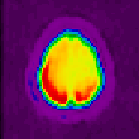
\includegraphics[width=0.17\textwidth]{figures/intro/full_pred.pdf}};
        \draw[->, ultra thick, draw=blue] ($(3rdoutnode)+(0,0.5)$) -- ($(1stprediction)+(0,-1.8)$);
        %x
        \node (input) at ($(2ndinnode)+(0,-2)$) {};
        \node (raw) at ($(input)+(-1.,0)$) {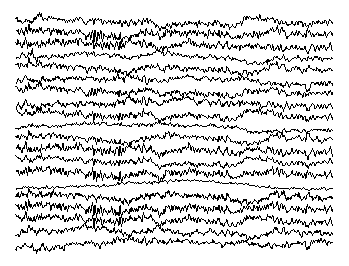
\includegraphics[width=0.08\textwidth]{figures/intro/eeg.pdf}};
        \node (stft) at ($(input)+(1.,0)$) {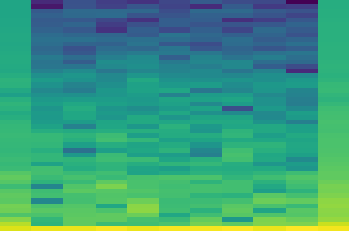
\includegraphics[width=0.09\textwidth]{figures/intro/stft.pdf}};
        \draw[->] ($(raw)+(0.7,0)$) -- ($(stft)+(-0.8,0)$);
        \draw[->, ultra thick, draw=blue] ($(input)+(0,1.1)$) -- ($(2ndinnode)+(0,-0.4)$);

        \node (eeg_legend) at ($(input)+(-3.5,0)$) {};
        \node[align=center] at ($(input)+(-3.7,0)$) {EEG recording\\Time frequency\\STFT domain};
        \node (model_legend) at ($(2ndinnode)+(-3.5,0.5)$) {Model};
        \node (fmri_legend) at ($(1stprediction)+(-3.5,0)$) {fMRI prediction};
        %table like lines
        \draw[dotted, opacity=0.8] ($(eeg_legend)+(-2,1.3)$) -- ($(eeg_legend)+(11.8,1.3)$);
        \draw[dotted, opacity=0.8] ($(model_legend)+(-2,1.15)$) -- ($(model_legend)+(11.8,1.15)$);

        
        
        %draw model 2nd 
        %in nodes
        \node (1stinnode) at ($(1stinnode)+(6.5,0)$) [in_node] {};
        \node (2ndinnode) at ($(1stinnode)+(0.5,0)$) [in_node] {};
        \node (3rdinnode) at ($(2ndinnode)+(0.5,0)$) [in_node] {};
        %out nodes
        \node (2ndoutnode) at ($(2ndinnode)+(0,1)$) [out_node] {};
        \node (3rdoutnode) at ($(2ndoutnode)+(0.5,0)$) [out_node] {};
        \node (1stoutnode) at ($(3rdoutnode)+(-1,0)$) [out_node] {};
        %fully connect nodes
        \draw[->] (1stinnode) -- (1stoutnode);
        \draw[->] (1stinnode) -- (2ndoutnode);
        \draw[->] (1stinnode) -- (3rdoutnode);
        \draw[->] (2ndinnode) -- (1stoutnode);
        \draw[->] (2ndinnode) -- (2ndoutnode);
        \draw[->] (2ndinnode) -- (3rdoutnode);
        \draw[->] (3rdinnode) -- (1stoutnode);
        \draw[->] (3rdinnode) -- (2ndoutnode);
        \draw[->] (3rdinnode) -- (3rdoutnode);
        %prediction
        \node (2ndprediction) at ($(2ndoutnode)+(0,2.8)$) {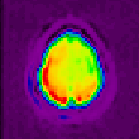
\includegraphics[width=0.17\textwidth]{figures/intro/relaxed_pred.pdf}};
        \draw[->, ultra thick, draw=blue] ($(2ndoutnode)+(0,0.5)$) -- ($(2ndprediction)+(0,-1.8)$);
        %eeg x
        \node (input) at ($(2ndinnode)+(0,-2)$) {};
        \node (raw) at ($(input)+(-1.,0)$) {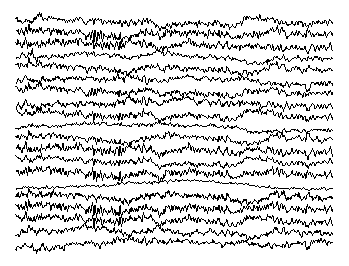
\includegraphics[width=0.08\textwidth]{figures/intro/eeg.pdf}};
        \node (stft) at ($(input)+(1.,0)$) {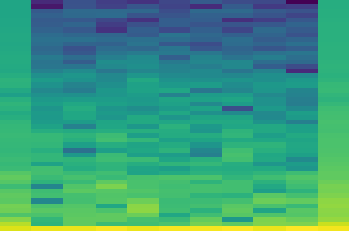
\includegraphics[width=0.09\textwidth]{figures/intro/stft.pdf}};
        \draw[->] ($(raw)+(0.7,0)$) -- ($(stft)+(-0.8,0)$);
        \draw[->, ultra thick, draw=blue] ($(input)+(0,1.1)$) -- ($(2ndinnode)+(0,-0.4)$);
        %problem relaxation
        \draw[->, ultra thick] ($(5thoutnode)+(0.5,0.5)$) -- ($(1stoutnode)+(-0.5,0.5)$);
        \node[align=center] (description) at ($(5thoutnode)+(2.45,-0.5)$) {predict less\\features};

        \node at ($(fmri_legend)+(0,2.1)$) {Resolution};
        \node at ($(1stprediction)+(0,2.1)$) {full};
        \node at ($(2ndprediction)+(0,2.1)$) {lower};
        \draw[opacity=0.4] ($(fmri_legend)+(-2,1.7)$) -- ($(fmri_legend)+(11.8,1.7)$);

        \node at ($(1stprediction)+(2.3,0.8)$) {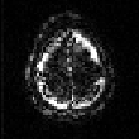
\includegraphics[width=0.065\textwidth]{figures/intro/full_res.pdf}};
        \node at ($(2ndprediction)+(-2.3,0.8)$) {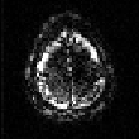
\includegraphics[width=0.065\textwidth]{figures/intro/relaxed_res.pdf}};
        
    \end{tikzpicture}
    \caption{EEG-to-fMRI synthesis and the spectral relaxation. EEG windows are transformed to the time--frequency (STFT) domain and mapped to an fMRI volume. The relaxed decoder predicts only the low spatial frequencies of the volume (fewer outputs, right) instead of the full resolution (left), consistent with the low spatial resolution of the EEG. The predictions are real outputs for a CHUR-XP2 test subject (axial slice 20): the stochastic spectral decoder, whose samples span the full resolution (left), and the zero-filled heteroscedastic network (right); the small grey maps beside them are their absolute residues; we also quantify what such a relaxed decoder can and cannot express.}
    \label{fig:idea_description}
\end{figure}


This study asks whether the uncertainty of EEG-to-fMRI synthesizers is about the EEG. To this end, our contributions are:
\begin{itemize}
	\item \textbf{An EEG-conditional evaluation protocol.} A model must beat EEG-free predictive distributions, and must change when its EEG is shifted in time or swapped across subjects (see Sec. \ref{sec:problem}).
	\item \textbf{A benchmark of eleven UQ methods} on a shared backbone, including our stochastic spectral decoder built on a DCT relaxation of the decoder. None beats an EEG-free template, and their uncertainty is a static anatomical map (see Sec. \ref{sec:methods}).
	\item \textbf{A positive control} showing that the heteroscedastic training most methods share makes the network ignore its input (see Sec. \ref{sec:results}).
	\item \textbf{A region-level analysis} in which an EEG model passes the surrogate test of \citet{mehta2025eegbold}, but heart rate from the in-scanner ECG predicts as much, and across subjects the EEG adds nothing to heart rate and motion (see Sec. \ref{sec:results}).
\end{itemize}
The results concern two motor-imagery datasets and the models we tested; they do not say that EEG carries no haemodynamic information \citep{goldman2002simultaneous,laufs2003eeg}.


\section{Methods}\label{sec:methodsall}

\textbf{Data and Ethics}. We use CHUR-XP2 (OpenNeuro ds002338) \citep{lioi2019simultaneous}: simultaneous EEG--fMRI from 17 healthy participants, motor-imagery run after neurofeedback training (\texttt{MIpost}), a block design with the same timing for every participant. EEG: 63 scalp channels and one ECG lead, corrected for gradient and pulse artefacts; fMRI: TR 1\,s, a 16-slice slab, resized to $64\times64\times30$. We replicate the main analyses on the motor-localizer run of CHUR-XP1 (ds002336; 9 subjects, TR 2\,s). Both public, de-identified datasets were acquired with ethical approval and informed consent \citep{lioi2019simultaneous}; this secondary analysis required no additional approval.

\subsection{EEG-conditional protocol}\label{sec:problem}

Each subject $s$ has pairs $(x_{s,t}, y_{s,t})$, where $y_{s,t}$ is the fMRI volume at time $t$ and $x_{s,t}$ the short-time Fourier magnitude of the EEG over the 10\,s before it. A synthesizer is a predictive distribution $p_\theta(y\mid x)$, trained and tested on disjoint subjects. We score it with the negative log-likelihood (NLL), the continuous ranked probability score (CRPS) \citep{gneiting2007strictly} and the root mean square error (RMSE) over a brain mask fixed from the training subjects, together with interval coverage, the Spearman correlation between predictive standard deviation (SD) and error, and sparsification (Supplementary Section~S2). Subjects, not volumes, are the unit of every test. A synthesizer is \emph{informative about the EEG} only if it passes two comparisons.

The \emph{EEG-free references} define the null hypothesis that a model uses no EEG information; we reject it only if the model scores better than all of these predictive distributions, which never see EEG:
\begin{itemize}
	\item \textbf{population template}: a voxelwise Gaussian distribution with the mean and standard deviation of all training volumes;
	\item \textbf{stimulus-locked template}: the same moments at each volume index, which predicts the task response without EEG;
	\item \textbf{own-subject oracle}: with the test subject's own voxel moments, an upper bound that uses test data.
\end{itemize}

We also compare the EEG based models with \emph{EEG nulls}. These models are evaluated with their input replaced by:
\begin{itemize}
	\item a \textbf{shift null}, the subject's EEG circularly shifted by at least 30 volumes, complementary to the IAAFT surrogates of \citet{mehta2025eegbold}, which randomize the phases of the BOLD instead;
	\item a \textbf{swap null}, another test subject's EEG at the same volume index.
\end{itemize}
We compare the median voxel temporal correlation $r$ between predicted and observed time courses. Beating the shift null but not the swap null means the model learned something locked to the shared task timing, not to the subject's EEG.

All comparisons use one-sided paired Wilcoxon tests over subjects at $\alpha=0.05$. Every claim of absence is backed by a Hodges--Lehmann estimate with a bootstrap 95\% confidence interval (CI) and a non-superiority test against a smallest effect of interest fixed in advance: $0.05$ in $r$, and 5\% of the template--oracle gap in NLL, CRPS and RMSE. Conformal intervals are calibrated on two held-out subjects per fold, and cross-conformally on all other subjects.

\subsection{Synthesizers}\label{sec:methods}
All networks share the encoder of \citet{calhas2022eeg}, whose architecture was found by neural architecture search \citep{calhas2021automatic} and is kept fixed. Only the decoder differs between methods.

\paragraph{Spectral relaxation.} We propose a low resolution prediction produced by the discrete cosine transform (DCT) \citep{ahmed1974discrete}, which pads the coefficients with zeros to full size and inverts the transform (Fig.~\ref{fig:upsampling_dct}). With a relaxation factor $\kappa=2$ it predicts $32\times32\times15$ instead of $64\times64\times30$ values, on the premise that EEG cannot inform the full resolution of the fMRI \citep{burle2015spatial}. Every output then lies in the span of the retained DCT basis, so the orthogonal projection onto that span gives an exact bound on what any relaxed decoder can express.

\begin{figure}[ht]
	\centering
	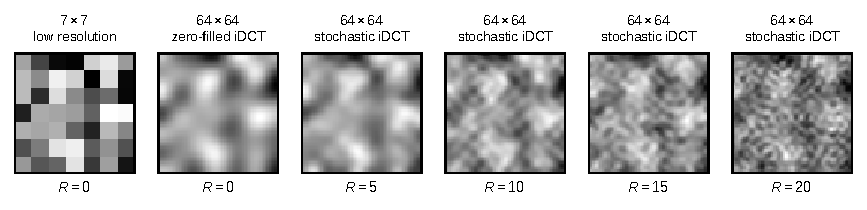
\includegraphics[width=\textwidth]{figures/dct_upsampling.pdf}
	\caption{Upsampling through the DCT, from $7\times 7$ to $64\times 64$. Left to right: the low-resolution image, its zero-filled upsampling, and upsamplings with an increasing number of Gaussian random coefficients above the cutoff.}
	\label{fig:upsampling_dct}
\end{figure}

\paragraph{Stochastic spectral decoder.} Our UQ method makes the relaxed decoder stochastic in the DCT domain (Fig.~\ref{fig:spectralUpsampling}). The retained coefficients are multiplied by Gaussian gains, and every coefficient above the cutoff is a sum of $H=20$ sinusoids of von Mises variables, weighted by an attention over the low coefficients. Its samples span the full resolution. Its noise parameters are trained by maximum likelihood without a prior, so we score it as a predictive distribution (Supplementary Section~S3).

\begin{figure*}[!htbp]
    \centering
    \begin{tikzpicture}[scale=3]
        \node (xaxis) at (3.2,0) {$r$};
        \node (yaxis) at (-0.1,1) {$p$};
        %axes
        \draw ($(xaxis)+(-3.2,0)$) -- ($(xaxis)+(-0.65,0)$);
        \node (dots) at ($(xaxis)+(-0.5,0)$)  {$\dots$};
        \draw[->]  ($(xaxis)+(-0.35,0)$) -- ($(xaxis)+(-0.1,0)$);
        \draw[->] ($(yaxis)+(0.1,-1.1)$) -- ($(yaxis)+(0.1,0)$);
        
        \node (origin) at (0,0) {};
        
        \draw[bottom color=blue,top color=blue!10, draw=blue] ($(origin)+(0.1,0)$) .. controls +(0,0) and +(0,0) .. ($(origin)+(0.1,0.5)$) .. controls +(0.5,0.5) and +(-0.2,0.5) .. ($(origin)+(1.5,0.5)$) .. controls +(0,0) and +(0,0) .. ($(origin)+(1.5,0)$);
        
        
        \draw[bottom color=yellow,top color=yellow!10, draw=orange] ($(origin)+(1.5,0)$) .. controls +(0,0) and +(0,0) .. ($(origin)+(1.5,0.5)$) .. controls +(0.4,-0.7) and +(-0.2,0.1) .. ($(origin)+(2.5,0)$);
        
        \node[rectangle, draw=blue] (X) at ($(origin)+(0.8, 0.45)$) {$X$};
        \node[rectangle, draw=orange] (C) at ($(origin)+(1.62, 0.12)$) {$C$};
        
        \node at ($(origin)+(0.1,-0.1)$) {$0$};
        \node at ($(origin)+(1.5,-0.1)$) {$N$};
        \node at ($(origin)+(2.5,-0.1)$) {$L$};
        \node at ($(origin)+(2.9,-0.1)$) {$M$};
        \draw ($(origin)+(0.1,0)$) -- +(0,-0.03);%referencing
        \draw ($(origin)+(1.5,0)$) -- +(0,-0.03);%referencing
        \draw ($(origin)+(2.5,0)$) -- +(0,-0.03);%referencing
        \draw ($(origin)+(2.9,0)$) -- +(0,-0.03);%referencing
        
        \node[rectangle, draw=orange, fill=yellow!50, text width=0.45\textwidth, minimum width=2, inner sep=3, align=left, anchor=west] (explain) at ($(origin)+(1.8,0.65)$) {\begin{gather*}
            W \in \mathbb{R}^{N \times H}: a = X \cdot W \\ 
            c^* \sim \mbox{vM}(\mu^*, \tau^*)^{R \times H}: C=\alpha \cdot \left[ b \odot \mbox{cos}(c^{*\top}) \right] 
        \end{gather*}};
        
        \node (x_tilde) at ($(origin)+(1.5, -0.3)$) {$\dot{\tilde{X}} = \begin{bmatrix} X_1 \odot c_1 & \dots & X_N \odot c_N & C_{1} & \dots & C_{R} & 0 & \dots & 0 \end{bmatrix} \in \mathbb{R}^{M}$};
    \end{tikzpicture}
    \caption{DCT coefficients of the stochastic spectral decoder in one dimension: the low block $X$, perturbed by the Gaussian gains $c$, the stochastic block $C$, and zeros up to $M$.}
    \label{fig:spectralUpsampling}
\end{figure*}

\paragraph{UQ methods.} The distributional methods use a Laplace likelihood whose log-scale is a smooth field linear in the latent, with $T=50$ stochastic passes. We compare split conformal on a point predictor, heteroscedastic Laplace \citep{kendall2017uncertainties}, deep evidential regression \citep{amini2020deep}, conformalized quantile regression \citep{romano2019conformalized}, MC dropout \citep{gal2016dropout}, MC spectral dropout \citep{khan2019regularization}, the stochastic spectral decoder, Flipout \citep{wen2018flipout} on the relaxed and the full-resolution decoder, SWAG-diagonal \citep{maddox2019simple}, last-layer Laplace \citep{daxberger2021laplace} and a five-member deep ensemble \citep{lakshminarayanan2017simple}. Every method, and every EEG-free reference, is then conformalized.

The EEG input is the 1--50\,Hz STFT of the 63 EEG channels (the ECG lead is dropped) in ten 1-s windows before each volume, 284 pairs per subject. Targets are the run standardized as a whole (\emph{run z-score}, mostly anatomy) and each voxel's z-scored time course (\emph{fluctuation}), in native space and registered to MNI space. The 17 subjects form five folds of 3--4 test, 2 calibration and 11--12 training subjects; every configuration is trained with three seeds (Adam, learning rate $2.98\times10^{-3}$, batch 4, 10 epochs); details and controls are in Supplementary Section~S2.

\subsection{Positive control}\label{sec:positive}
A negative result needs a pipeline that could have produced a positive one. We add a known EEG-coupled signal to an $8\times8\times4$-voxel box of every subject's fluctuation target: the negated C3/C4 8--30\,Hz power of the models' own input, convolved with a canonical HRF, with variance $s\in\{0.1,0.3,1\}$ relative to the fluctuations. We ask which models recover it: a kernel ridge on the band power of the input window (\emph{linear probe}), a linear map and an MLP on the same features, and the backbone with the heteroscedastic head, a point $L_1$ loss, or the heteroscedastic head at a lower learning rate ($10^{-4}$, batch 32, 30 epochs).

\subsection{Region-level ridge with physiological confounds}\label{sec:ridge}
We also fit a model of the kind reported to work: lagged, linear and at the region scale. A ridge regression \citep{hoerl1970ridge} on the log band power of the 63 EEG channels in five bands at lags of 0--19\,s predicts a registered sensorimotor ROI time course, within subjects and across subjects. Heart rate from R peaks of the in-scanner ECG, the ECG band power and the motion parameters are fitted in exactly the same way, and nested models ask whether the EEG adds to heart rate and motion (held-out $\Delta R^2$). Each model is tested against 100 IAAFT surrogates of the BOLD \citep{schreiber1996improved} and the swap null, and we replicate the pipeline and test of \citet{mehta2025eegbold}.


\FloatBarrier
\section{Results}\label{sec:results}
At $\kappa=2$ the retained block holds 97.9\% of the energy of a volume but only 33\% of a voxel's temporal variance (Fig.~\ref{fig:oracle}). The relaxation lowers the voxel error because it keeps the static anatomy, and for the same reason it cannot express two thirds of the dynamics that an EEG could inform.

\begin{figure}[ht]
	\centering
	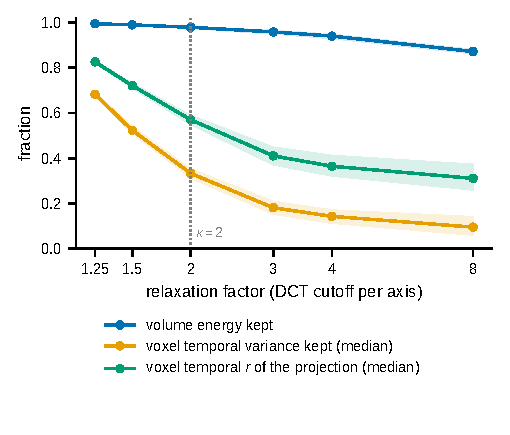
\includegraphics[width=0.55\textwidth]{figures/oracle_bound.pdf}
	\caption{Oracle projection onto the retained DCT block: the volume energy is almost entirely kept, but most of each voxel's temporal variance is not. Lines: mean over subjects; bands: range over subjects.}
	\label{fig:oracle}
\end{figure}

\begin{table}[!htbp]
	\centering
	\caption{UQ benchmark on CHUR-XP2, run-z-score target (17 test subjects; seeds averaged). Lower is better for RMSE ($\pm$ SD over seeds), NLL, CRPS and AUSE. PICP$_{90}$: coverage of the model's own 90\% interval; Conf$_{90}$: of the per-voxel split-conformal 90\% interval; $\rho$: Spearman correlation between predictive SD and absolute error. Last three columns: one-sided paired Wilcoxon $p$ for NLL below the population template, and median voxel $r$ above the shift and swap nulls (bold: $p<0.05$). The own-subject oracle uses test data. $^\dagger$Diverged in every seed.}
	\label{tab:uq}
	\setlength{\tabcolsep}{3pt}
	\resizebox{\textwidth}{!}{%
	\begin{tabular}{lcccccccccc}
		\toprule
		Method & RMSE & NLL & CRPS & PICP$_{90}$ & Conf$_{90}$ & $\rho$ & AUSE & $p_{\mathrm{NLL}<\mathrm{tmpl}}$ & $p_{r>\mathrm{shift}}$ & $p_{r>\mathrm{swap}}$\\
		\tabinput{tables/uq_benchmark}
		\bottomrule
	\end{tabular}}
\end{table}

The population template, which never sees EEG, has an NLL of 0.463, a CRPS of 0.239 and an RMSE of 0.520 (Table~\ref{tab:uq}). Our results show that no method is significantly better on any of the three. The deep ensemble comes closest (NLL 0.393, $p=0.23$), mostly through mixing: its members average 0.522. For every single-model method an NLL gain of at least the smallest effect of interest is rejected (Supplementary Table~S1).

\begin{figure}[!htbp]
	\centering
	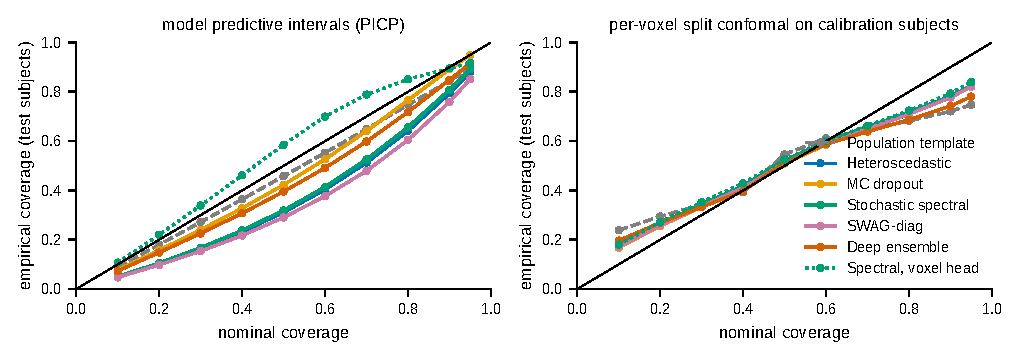
\includegraphics[width=\textwidth]{figures/reliability.pdf}
	\caption{Reliability on test subjects (run-z-score target). Left: coverage of each model's own central intervals. Right: after per-voxel split conformal calibration on two held-out subjects. The EEG-free template (dashed) is as well calibrated as any network.}
	\label{fig:reliability}
\end{figure}
The usual diagnostics do not separate the networks from the template either (Fig.~\ref{fig:reliability}): the template is as well calibrated, and its spread tracks its error better ($\rho=0.52$ vs 0.47--0.51). After conformal calibration on two subjects every method, the template included, under-covers (72--79\% at 90\%); calibrating on all 16 other subjects restores 88--90\% (Supplementary Table~S6).

\textbf{Predicted uncertainty does not depend on the EEG}\label{sec:res:nulls}
\begin{figure}[!htbp]
	\centering
	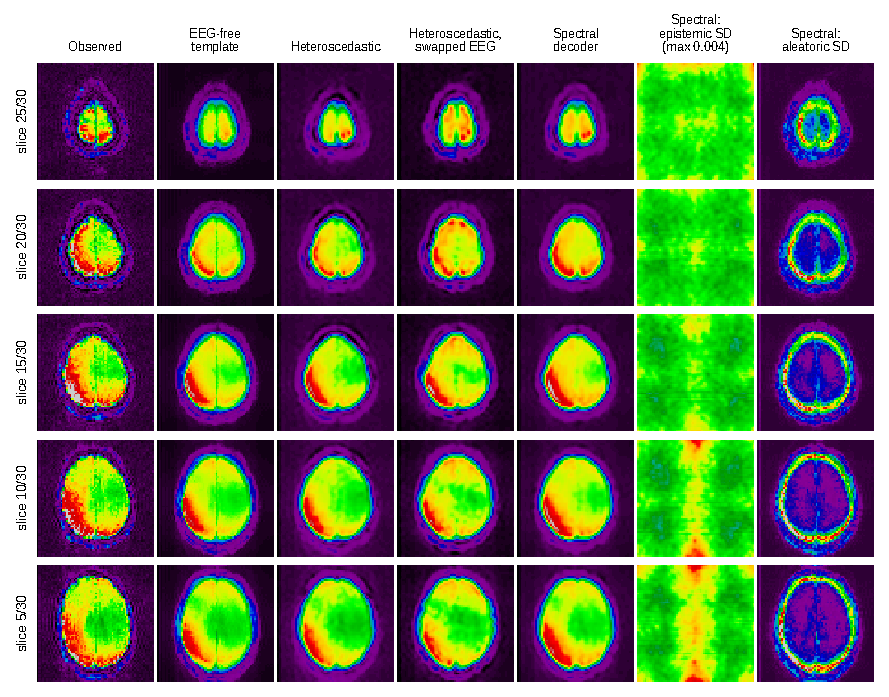
\includegraphics[width=\textwidth]{figures/volumes.pdf}
	\caption{Synthesized volumes for one CHUR-XP2 test subject (first test volume, fold 0, seed 2). From left: the observed volume; the EEG-free population template; the heteroscedastic network with the subject's EEG and with another subject's EEG; the stochastic spectral decoder's prediction, and its epistemic and aleatoric predictive SD (own colour scales). The predictions reproduce the template whatever EEG is given, and the aleatoric SD follows the anatomy. The epistemic SD is a mirror-symmetric pattern set by the DCT basis (Section~\ref{sec:res:nulls}).}
	\label{fig:volumes}
\end{figure}
No method's temporal correlation exceeds the subject-swap null, and an EEG-specific gain of $\delta_r=0.05$ is rejected for every method ($p<0.001$). All are below $r=0.016$, against 0.160 for the stimulus-locked template. The predictive spread is a fixed map (Fig.~\ref{fig:volumes}): its variance over time is $10^{-6}$ to $10^{-3}$ of its variance across voxels, the SD maps under the real, shifted and swapped EEG correlate at $1.000$, and the spread tracks the anatomical part of the error ($\rho\approx0.5$), not its temporal part (Supplementary Table~S2).

The epistemic map of the stochastic spectral decoder has no anatomy for a structural reason. Its noise enters as independent DCT coefficients $Z_k$, so its epistemic variance at voxel $v$ is $\sum_k \mathrm{Var}[Z_k]\,\phi_k(v)^2$; each squared basis function $\phi_k^2$ is unchanged by reflecting $v$ about the centre of the field of view, so the map is mirror-symmetric whatever variances are learned. Anatomy could enter only through the gains on the retained coefficients, which shrank in training (epistemic variance $4\times10^{-6}$, aleatoric 0.26). In Fig.~\ref{fig:volumes}, 73\% of the map's spatial variance is mirror-symmetric and the rest is within the Monte Carlo error of 50 samples: noise in a global basis gives global, symmetric uncertainty.

\begin{table}[!htbp]
	\centering
	\caption{Positive control: median voxel $r$ in the injected box, mean over 17 test subjects, shift and swap nulls in brackets. Ceiling: $\sqrt{s/(1+s)}$. Ridge: kernel ridge on band power of the input window. Linear and MLP: the same features with the deep models' loop (Laplace likelihood, Adam at $2.98\times10^{-3}$, batch 4, 10 epochs) or a regression loop (MSE, batch 64, 50 epochs). Backbone: heteroscedastic head, point $L_1$ loss, and heteroscedastic head at learning rate $10^{-4}$. --: not run.}
	\label{tab:positive}
	\setlength{\tabcolsep}{3pt}
	\resizebox{\textwidth}{!}{%
	\begin{tabular}{cccccccccc}
		\toprule
		$s$ & ceiling & ridge & linear, deep loop & linear, MSE & MLP, deep loop & MLP, MSE & backbone, hetero. & backbone, $L_1$ & backbone, hetero., lr $10^{-4}$\\
		\midrule
		\tabinput{tables/positive_control}
		\bottomrule
	\end{tabular}}
\end{table}
The linear probe recovers the injected signal at every strength ($r=0.59$ at $s=1$, ceiling 0.71; nulls near zero), while the heteroscedastic backbone, the base of most UQ methods, recovers it at none (Table~\ref{tab:positive}). The same backbone recovers it with a point loss ($r=0.48$) or a lower learning rate ($0.49$), and a linear map and an MLP lose it when trained with the deep models' loop: at the searched learning rate the learned variance absorbs the residual and the mean stops fitting \citep{seitzer2022pitfalls}.

\begin{figure}[!htbp]
	\centering
	\begin{subfigure}[t]{\textwidth}
		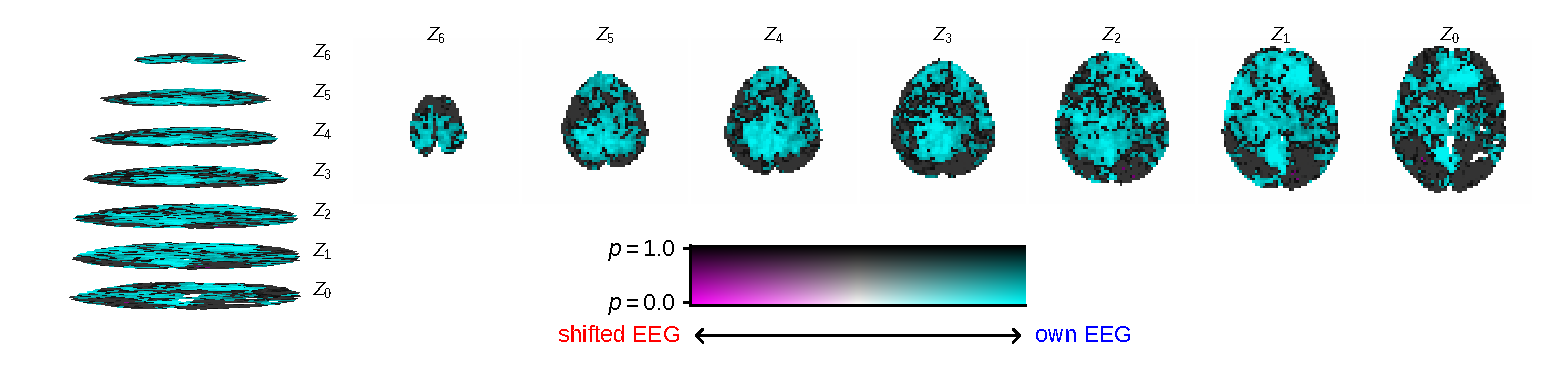
\includegraphics[width=\textwidth]{figures/sig_mni_hetero_lr1e-4_b32_fluct_real_vs_shift.pdf}
		\caption{Own EEG vs EEG shifted in time.}
	\end{subfigure}
	\begin{subfigure}[t]{\textwidth}
		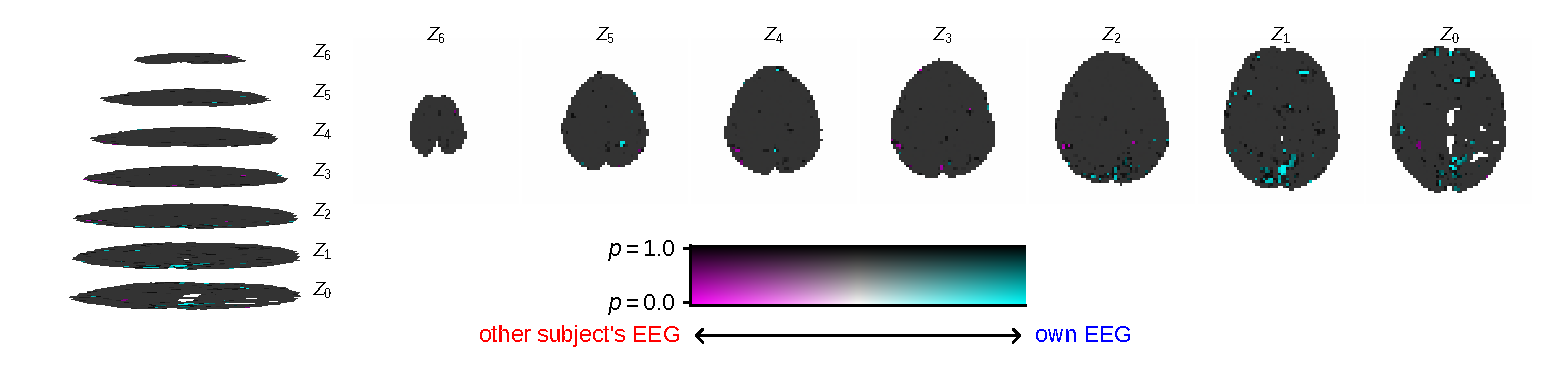
\includegraphics[width=\textwidth]{figures/sig_mni_hetero_lr1e-4_b32_fluct_real_vs_swap.pdf}
		\caption{Own EEG vs another subject's EEG.}
	\end{subfigure}
	\begin{subfigure}[t]{\textwidth}
		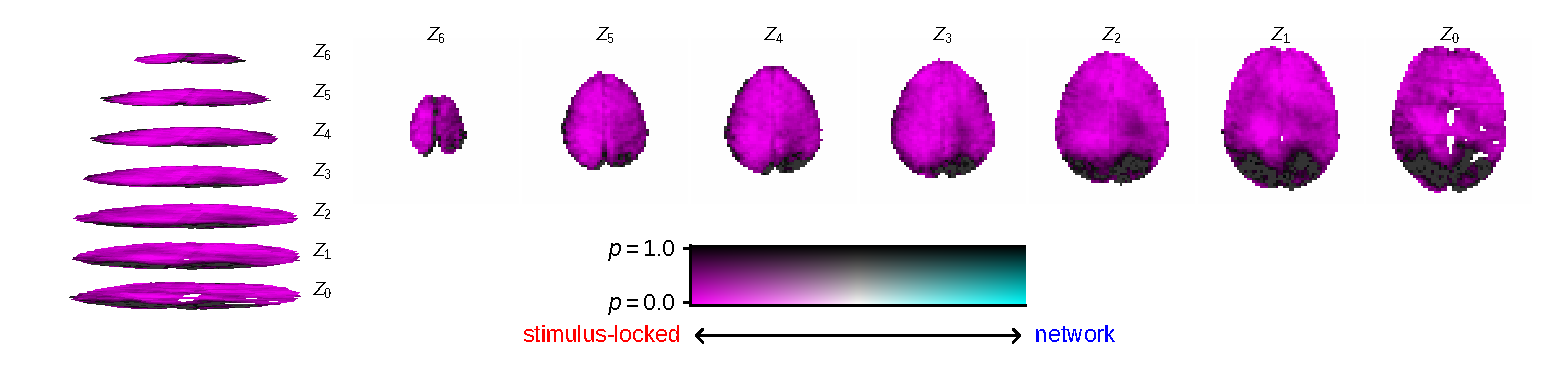
\includegraphics[width=\textwidth]{figures/sig_mni_hetero_fluct_vs_locked.pdf}
		\caption{Network vs EEG-free stimulus-locked template.}
	\end{subfigure}
	\caption{Where does the EEG help? Voxelwise paired Wilcoxon tests over the 17 CHUR-XP2 subjects of the temporal correlation between predicted and observed fluctuations, registered volumes; 13{,}785 brain voxels (mean registered EPI above half its range, all tested). Seven axial slices from the lowest slice fully inside the oblique acquisition slab ($Z_0$) to near the vertex ($Z_6$), 3-D stack at left. Grey: $p\ge0.05$; coloured: the condition named at that end of the colour bar is significantly better, brighter for larger $r$. (a, b) The heteroscedastic network at the lower learning rate, which recovers an injected signal: its own EEG beats the shifted EEG in 50\% of the voxels (cyan), but differs from another subject's EEG in 1.6\% (187 better, 30 worse), fewer than expected by chance. (c) The stimulus-locked template beats the network in 90\% of the voxels (magenta).}
	\label{fig:sigmaps}
\end{figure}
Trained with the recipes that recover the injected signal, the networks on the real fluctuations exceed the time-shift null ($r=0.030$--$0.066$, $p\le0.022$) but not the subject-swap null ($p\ge0.37$), and so does the linear probe (Fig.~\ref{fig:sigmaps}). The stimulus-locked template, which only knows when the imagery blocks occur, beats them almost everywhere. A network given only the ECG lead scores about as well as one given the EEG, and removing the task-locked response leaves nothing predictable (Supplementary Section~S4).


\begin{figure}[!htbp]
	\centering
	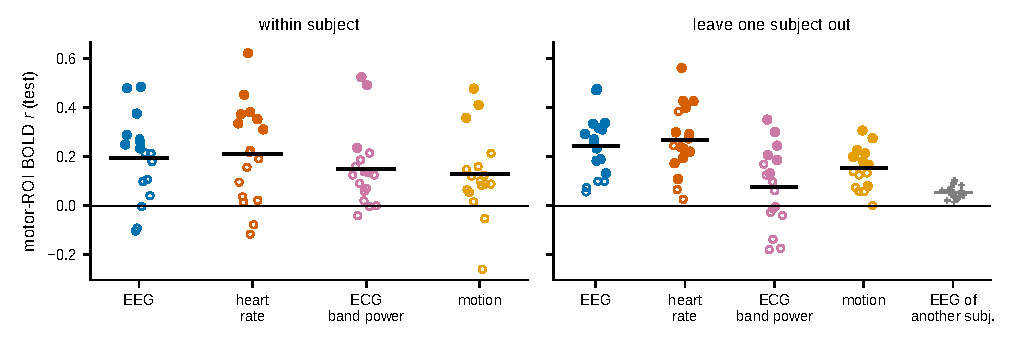
\includegraphics[width=\textwidth]{figures/ridge.pdf}
	\caption{ROI ridge across subjects, task regressed out: test correlation per subject for EEG, heart rate, ECG band power and head motion (filled: above the subject's IAAFT surrogates at $p<0.05$), and the EEG model scored on another subject's EEG. Black bars: means.}
	\label{fig:ridge}
\end{figure}
\begin{table}[!htbp]
	\centering
	\caption{Nested models: does the EEG add to the physiological confounds? Held-out $R^2$ of the confounds alone and with the EEG, task regressed out; $\Delta R^2$ with the one-sided Wilcoxon $p$ of a gain, and $\Delta R^2$ with another subject's EEG.}
	\label{tab:nested}
	\small
	\begin{tabular}{llcccccc}
		\toprule
		Design & confounds & $n$ & $R^2$ reduced & $R^2$ full & $\Delta R^2$ & $p_{\Delta>0}$ & $\Delta R^2$ swap\\
		\midrule
		\tabinput{tables/ridge_nested}
		\bottomrule
	\end{tabular}
\end{table}
\textbf{At the region level, heart rate predicts as much as the EEG.} Within subjects the EEG and heart-rate ridges each beat their surrogates in 7 of 17 subjects, but no model beats the block design. Across subjects the EEG ridge looks like a success: with the task regressed out it reaches $r=0.243$, 13 of 17 subjects beat their surrogates (binomial $p<0.001$), and it beats the swap null ($p<0.001$; Fig.~\ref{fig:ridge}), although not the block design ($p=0.066$). But heart rate alone predicts the same region as well ($r=0.268$, 13 of 17; EEG not better, $p=\ridgeEEGvsHR$), and in nested models the EEG adds nothing to heart rate and motion across subjects ($\Delta R^2=-0.001$, $p=0.50$; Table~\ref{tab:nested}). Within subjects it adds a small amount ($\Delta R^2=0.028$, $p=0.044$, uncorrected) that does not survive adding the ECG band power to the confounds ($\Delta R^2=0.013$, $p=0.15$). The EEG also still carries the heart: after pulse-artefact correction, 20\% of its band-power features correlate with heart rate at $|r|>0.2$, against 1.7\% with a shifted heart rate ($p<0.001$).

The pipeline and test of \citet{mehta2025eegbold}, applied as published, also support EEG-to-BOLD prediction here (trial-evoked $r=0.182$ within runs, 8 of 16 subjects beyond surrogates, binomial $p<0.001$, better than both of their reference models, FDR-corrected $p=0.005$), and the same pipeline on the ECG lead alone does nearly as well ($r=0.149$, 9 of 16; Supplementary Table~S10).

\subsection{Replication on CHUR-XP1}\label{sec:res:xp1}
On CHUR-XP1 the voxel-level results and the positive control replicate (Supplementary Table~S4). No model exceeds the swap null, the predicted SD maps under real and null EEG correlate at 1.000, and the point-loss backbone recovers the injected signal ($r=0.37$) while the heteroscedastic one does not ($r=-0.02$). Two methods have a lower NLL than the template (ensemble $p=0.004$, stochastic spectral decoder $p=0.020$) but none a lower CRPS or RMSE, which we read as a calibration effect of six or seven training subjects. At the region level the EEG ridge again predicts the ROI across subjects ($r=0.172$, 7 of 9), heart rate nearly as well ($r=0.137$; EEG not better, $p=0.18$), and the EEG adds nothing to heart rate and motion ($\Delta R^2=-0.005$, $p=0.54$).


\FloatBarrier
\section{Discussion}\label{sec:discussion}
\paragraph{Calibration is not informativeness.} A predictive distribution can be calibrated, sharp and correlated with its own errors without using its input. In EEG-to-fMRI synthesis this is the default, because anatomical variability decides both where errors occur and where any model is uncertain. All eleven methods learn this structure, and so does the EEG-free template, which none of them beats.

\paragraph{Heteroscedastic training can blind a synthesizer to its input.} A heteroscedastic likelihood can explain a residual by widening its variance instead of moving its mean, and with a weakly informative input and a high learning rate it does \citep{seitzer2022pitfalls}. Here this blinded a backbone that otherwise recovers an injected EEG signal, while its calibration stayed respectable; only a positive control reveals it.

\paragraph{What the EEG predicts physiology.} At the voxel level, models that can see an EEG-coupled signal find only the shared task timing. At the region level a lagged linear model predicts motor BOLD as convincingly as published results, but heart rate predicts it as well, the EEG adds nothing to heart rate and motion across subjects and at most a small within-subject increment that does not survive the ECG, and the EEG still contains cardiac signal after artefact correction. The simplest reading is physiological: heart-rate fluctuations drive BOLD changes and enter the EEG through residual pulse artefacts and autonomic covariation. EEG--BOLD coupling exists \citep{goldman2002simultaneous,laufs2003eeg}, but in these data a predictive model cannot separate it from physiology, and a surrogate test over the BOLD cannot either.

\paragraph{EEG-free references need to be used as nulls in EEG-to-fMRI synthesis.} We suggest: report EEG-free predictive distributions, including a stimulus-locked one, next to every model; claim EEG-specific information only above a subject-swap null; test whether the predicted uncertainty changes with the input; show with a positive control that the model, trained as reported, recovers a known input-coupled signal; test the EEG's increment over heart-rate and motion models; and back every claim of absence with an effect size.

\paragraph{Limitations.} The analyses use two motor-imagery datasets from one laboratory (17 and 9 subjects) with block designs, and tests with $n=17$ have limited power, although the equivalence tests bound what we could have missed. The positive control injects a linear, spatially fixed signal, and we did not retune every method's learning rate. Respiration was not recorded and may account for part of what we attribute to heart rate.

\section{Conclusions}\label{sec:conclusion}
We asked whether the uncertainty of EEG-to-fMRI synthesizers is about the EEG. On these data it is not: eleven UQ methods are not better than an EEG-free template, and their uncertainty is a static anatomical map. A positive control shows that heteroscedastic training makes the network ignore its input, and at the region level heart rate predicts as much as the EEG, which adds nothing to heart rate and motion across subjects. EEG-free references, subject-swap nulls, physiological confounds and positive controls are needed to show that a synthesizer uses neural information.


\section*{Declaration of the use of AI}
\emph{Tools.} Claude Opus 5.5 (Anthropic; model identifier \texttt{claude-opus-5-5}), used through the Claude Code command-line tool, version 2.1.299.

\emph{Research.} The AI assistant debugged analysis code (model training and evaluation scripts, the EEG-conditional evaluation, the ridge, linear-probe and replication analyses, and the scripts that generate every table and figure from the saved results), and ran and monitored the computations on the authors' computing cluster under their supervision. The authors designed the study, wrote the article and checked the code.

\emph{Figures.} All figures were produced by the analysis code from the saved results, or drawn in TikZ; no figure or data was generated by an AI image or data model.

\emph{Writing.} We used AI to review and insert table results. The authors reviewed and edited all text, checked every reference, and take full responsibility for the content.

\section*{Data and Code Availability}
Both datasets are public on OpenNeuro: CHUR-XP2 (ds002338) and CHUR-XP1 (ds002336) \citep{lioi2019simultaneous}. Code for all models, the EEG-free references, the evaluation (with its NumPy reference implementation and equivalence test), the oracle bound, the registration, the positive control and linear probe, the ROI ridge and nested confound models, and the replication of Mehta et al.\ is available at \url{https://github.com/DCalhas/eeg_to_fmri} (branch \texttt{uncertainty-journal}), commit \texttt{b6765b3}. Experiments used TensorFlow 2.9.3 and TensorFlow Probability 0.17.0 on NVIDIA A100 GPUs. The BOLD preprocessing and registration used FSL and nilearn. Every table and figure in this paper is generated from saved per-run summaries by \texttt{make\_tables.py} and \texttt{make\_figures.py}.


\section*{Author Contributions}
D.C.: Conceptualization, Methodology, Software, Formal analysis, Investigation, Data curation, Visualization, Funding acquisition, Writing -- original draft, Writing -- review \& editing. R.H.: Conceptualization, Methodology, Supervision, Funding acquisition, Writing -- review \& editing.

\section*{Funding}
This work was supported by national funds through Funda\c{c}\~{a}o para a Ci\^{e}ncia e Tecnologia (FCT), under the Ph.D.\ Grant SFRH/BD/5762/2020 to David Calhas. This research was supported by the Slovenian Research and Innovation Agency (ARIS) under the Artificial Intelligence and Intelligent Systems Programme (Grant No.~P2-0209) and by the European project 22HLT05 MAIBAI. This publication is co-funded by the European Union's Horizon Europe research and innovation programme under the Marie Sk{\l}odowska-Curie COFUND Postdoctoral Programme grant agreement No.~101081355-SMASH and by the Republic of Slovenia and the European Union from the European Regional Development Fund. Views and opinions expressed are however those of the author(s) only and do not necessarily reflect those of the European Union or the European Research Executive Agency. Neither the European Union nor the granting authority can be held responsible for them.

\section*{Declaration of Competing Interests}
The authors declare no competing interests.

\section*{Acknowledgements}
We thank the authors of the CHUR-XP1 and CHUR-XP2 datasets for making them public. Computations were performed on the Frida high-performance computing cluster of the Faculty of Computer and Information Science, University of Ljubljana.

\section*{Supplementary Material}
Supplementary Material (extended related work and methods, the stochastic spectral decoder, and Supplementary Tables S1--S11 and Figures S1--S3) is provided as a separate file.

\printbibliography

\end{document}
